\documentclass[UTF8]{ctexart}
\usepackage{ctex}
\usepackage{amsmath}
\usepackage{amsthm}
\usepackage{geometry}
\geometry{left=2.5cm,right=2.5cm,top=2.5cm,bottom=2.5cm}
\usepackage{amssymb}
\usepackage{indentfirst}
\usepackage{graphicx}
\usepackage{subfigure}
\usepackage{listings}
\usepackage{xcolor}
\usepackage{float}
\usepackage{algorithm}  
\usepackage{algorithmicx}  
\usepackage{longtable}
\usepackage{fancyhdr}
\usepackage{appendix}
\usepackage{enumitem}
\usepackage{abstract}
\usepackage{multirow}
\pagestyle{fancy}
\lfoot{}%这条语句可以让页码出现在下方
\theoremstyle{plain}
\newtheorem{thm}{Theorem}[section]
\newtheorem{lem}[thm]{Lemma}
\newtheorem{prop}[thm]{Proposition}
\newtheorem{cor}[thm]{Corollary}

\theoremstyle{definition}
\newtheorem{defn}{Definition}[section]

\theoremstyle{remark}
\newtheorem*{rem}{Remark}
\newtheorem{eg}{Example}[section]
\title{Project2}
\author{Shuang Hu}
\begin{document}
\maketitle
\section{Problem Statement}

Write a C++ Package to solve the BVP such as:
$$
\left\{
\begin{aligned}
-u''(x)&=f(x);\\
u(0)&=u_{0};\\
u(1)&=u_{1}.\\
\end{aligned}
\right.
$$
specially, I should use \textbf{multigrid method} to solve this problem, including VCycle and FMG cycle(Full Multigrid Cycle).
\section{Nonhomogenious test case}
In this test case, I set 
$$
\begin{aligned}
f(x)&=\sin xe^{\sin x}-\cos^{2}xe^{\sin x};\\
u_{0}&=1;\\
u_{1}&=e^{\sin(1)}.\\
\end{aligned}
$$
The actual solution of this problem is
$$
u(x)=\exp(\sin(x)).
$$

The result is shown as below:
\begin{figure}[H]
\centering
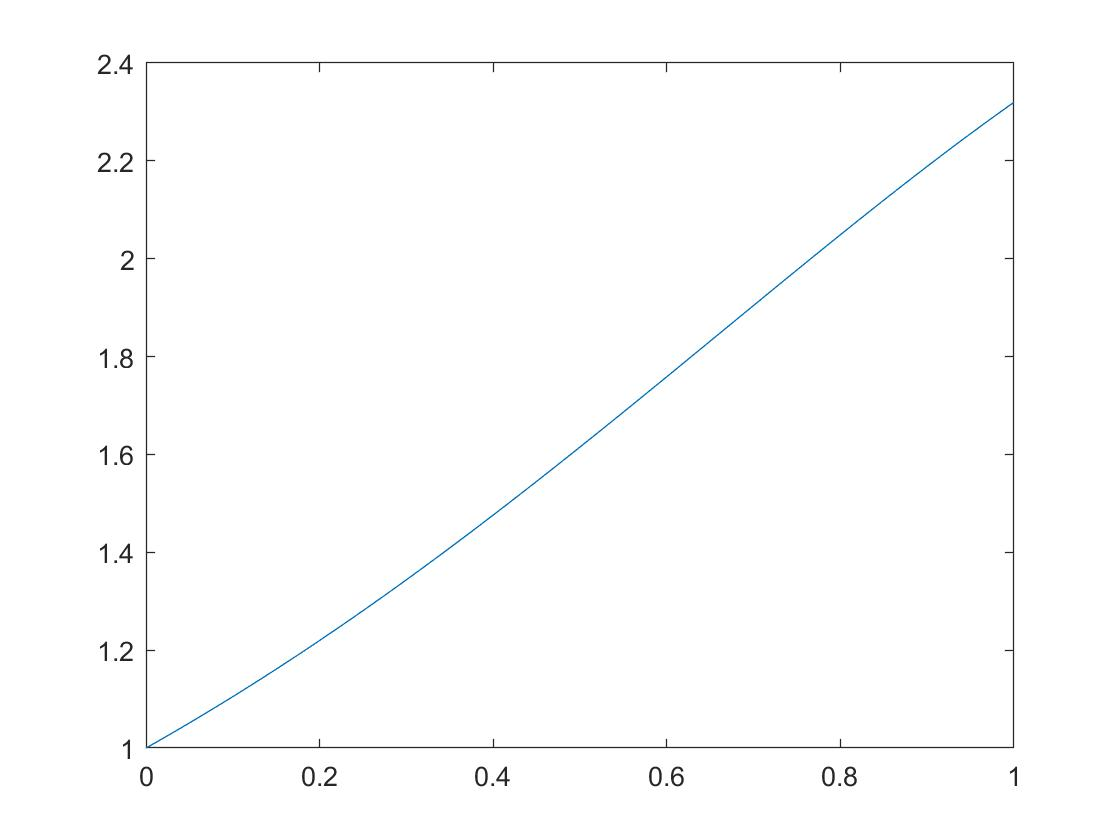
\includegraphics[height=0.2\textheight,width=0.5\linewidth]{1}
\caption{Result for test case 1.}
\end{figure}

Then, I test the convergence rate of V-Cycle method as $n=128,256,512,1024.$ Remark: I use relative error of solving the linear equations to measure the reduction rate.

Here are the convergence tables:
\begin{table}[H]
\centering
\begin{tabular}{|l|l|l|}
\hline
cycletimes & error & ratio\\\hline
1 & 0.0666637& \\ \hline
2 & 0.0113094& 5.89455\\ \hline
3 & 0.00181142& 6.24337\\ \hline
4 & 0.000290501& 6.23552\\ \hline
5 & 4.70991e-05& 6.16785\\ \hline
6 & 7.7282e-06& 6.09445\\ \hline
7 & 1.28214e-06& 6.02759\\ \hline
8 & 2.14797e-07& 5.96907\\ \hline
9 & 3.85331e-08& 5.57435\\ \hline
10 & 6.95844e-09& 5.5376\\ \hline
11 & 1.26092e-09& 5.51853\\ \hline
12 & 2.29349e-10& 5.49783\\ \hline
13 & 4.18761e-11& 5.47685\\ \hline
14 & 7.67467e-12& 5.4564\\ \hline
15 & 1.41128e-12& 5.43811\\ \hline
16 & 2.60591e-13& 5.41568\\ \hline
17 & 4.81037e-14& 5.41727\\ \hline
18 & 9.052e-15& 5.31415\\ \hline
19 & 1.77767e-15& 5.09207\\ \hline
20 & 5.05395e-16& 3.51738\\ \hline
21 & 5.74813e-16& 0.879235\\ \hline
22 & 5.18072e-16& 1.10952\\ \hline
23 & 5.18072e-16& 1\\ \hline
24 & 5.18072e-16& 1\\ \hline
25 & 5.18072e-16& 1\\ \hline
26 & 5.18072e-16& 1\\ \hline
27 & 5.18072e-16& 1\\ \hline
28 & 5.18072e-16& 1\\ \hline
29 & 5.18072e-16& 1\\ \hline
30 & 5.18072e-16& 1\\ \hline
31 & 5.18072e-16& 1\\ \hline
32 & 5.18072e-16& 1\\ \hline
\end{tabular}
\caption{The convergence rate of test case 1: n=128}
\end{table}
\begin{table}[H]
\centering
\begin{tabular}{|l|l|l|}
\hline
cycletimes & error & ratio\\\hline
1 & 0.0666665& \\ \hline
2 & 0.0113086& 5.89522\\ \hline
3 & 0.00181042& 6.24639\\ \hline
4 & 0.000290102& 6.24061\\ \hline
5 & 4.69854e-05& 6.17431\\ \hline
6 & 7.70041e-06& 6.10168\\ \hline
7 & 1.27592e-06& 6.03517\\ \hline
8 & 2.13481e-07& 5.97675\\ \hline
9 & 3.77894e-08& 5.64923\\ \hline
10 & 6.80175e-09& 5.55583\\ \hline
11 & 1.22867e-09& 5.53585\\ \hline
12 & 2.22829e-10& 5.51396\\ \hline
13 & 4.05763e-11& 5.49162\\ \hline
14 & 7.41863e-12& 5.46951\\ \hline
15 & 1.36183e-12& 5.44754\\ \hline
16 & 2.50937e-13& 5.42699\\ \hline
17 & 4.6485e-14& 5.39824\\ \hline
18 & 8.58091e-15& 5.41725\\ \hline
19 & 1.49783e-15& 5.72888\\ \hline
20 & 4.86884e-16& 3.07637\\ \hline
21 & 4.98337e-16& 0.977017\\ \hline
22 & 6.31191e-16& 0.789518\\ \hline
23 & 6.31191e-16& 1\\ \hline
24 & 5.73498e-16& 1.1006\\ \hline
25 & 5.32641e-16& 1.07671\\ \hline
26 & 4.82921e-16& 1.10296\\ \hline
27 & 5.1089e-16& 0.945254\\ \hline
28 & 4.49984e-16& 1.13535\\ \hline
29 & 5.32641e-16& 0.844818\\ \hline
30 & 4.82921e-16& 1.10296\\ \hline
31 & 4.82921e-16& 1\\ \hline
32 & 5.73498e-16& 0.842063\\ \hline
\end{tabular}
\caption{Convergence rate of test case 1: n=256}
\end{table}
\begin{table}[H]
\centering
\begin{tabular}{|l|l|l|}
\hline
cycletimes & error & ratio\\
\hline
1 & 0.0666667& \\ \hline
2 & 0.0113083& 5.89538\\ \hline
3 & 0.00181021& 6.24694\\ \hline
4 & 0.000290041& 6.24125\\ \hline
5 & 4.69729e-05& 6.17463\\ \hline
6 & 7.69876e-06& 6.10136\\ \hline
7 & 1.2759e-06& 6.034\\ \hline
8 & 2.13554e-07& 5.97458\\ \hline
9 & 3.76981e-08& 5.66486\\ \hline
10 & 6.78485e-09& 5.55621\\ \hline
11 & 1.22564e-09& 5.53578\\ \hline
12 & 2.22297e-10& 5.51351\\ \hline
13 & 4.04851e-11& 5.49083\\ \hline
14 & 7.40307e-12& 5.46869\\ \hline
15 & 1.35906e-12& 5.44721\\ \hline
16 & 2.50262e-13& 5.43054\\ \hline
17 & 4.63827e-14& 5.39559\\ \hline
18 & 8.66984e-15& 5.34989\\ \hline
19 & 1.58671e-15& 5.46402\\ \hline
20 & 6.0427e-16& 2.62583\\ \hline
21 & 7.283e-16& 0.8297\\ \hline
22 & 6.14868e-16& 1.18448\\ \hline
23 & 7.16439e-16& 0.858228\\ \hline
24 & 7.16439e-16& 1\\ \hline
25 & 7.16439e-16& 1\\ \hline
26 & 5.4544e-16& 1.31351\\ \hline
27 & 6.06313e-16& 0.899602\\ \hline
28 & 6.14868e-16& 0.986087\\ \hline
29 & 7.16439e-16& 0.858228\\ \hline
30 & 7.16439e-16& 1\\ \hline
31 & 7.16439e-16& 1\\ \hline
32 & 5.4544e-16& 1.31351\\ \hline
\end{tabular}
\caption{Convergence rate of test case 1: n=512}
\end{table}
\begin{table}[H]
\centering
\begin{tabular}{|l|l|l|}
\hline
cycletimes & error & ratio\\\hline
1 & 0.0666667&\\ \hline
2 & 0.0113082& 5.89541\\ \hline
3 & 0.00181018& 6.24702\\ \hline
4 & 0.000290034& 6.24127\\ \hline
5 & 4.6973e-05& 6.17448\\ \hline
6 & 7.69933e-06& 6.10092\\ \hline
7 & 1.27616e-06& 6.03319\\ \hline
8 & 2.13642e-07& 5.97336\\ \hline
9 & 3.77174e-08& 5.66429\\ \hline
10 & 6.79086e-09& 5.55414\\ \hline
11 & 1.22727e-09& 5.53331\\ \hline
12 & 2.22707e-10& 5.51068\\ \hline
13 & 4.05822e-11& 5.4878\\ \hline
14 & 7.42531e-12& 5.46539\\ \hline
15 & 1.36387e-12& 5.44428\\ \hline
16 & 2.51438e-13& 5.42429\\ \hline
17 & 4.64102e-14& 5.41774\\ \hline
18 & 8.69728e-15& 5.33617\\ \hline
19 & 1.61415e-15& 5.38815\\ \hline
20 & 7.58254e-16& 2.12877\\ \hline
21 & 6.56752e-16& 1.15455\\ \hline
22 & 7.26131e-16& 0.904454\\ \hline
23 & 6.91684e-16& 1.0498\\ \hline
24 & 6.56752e-16& 1.05319\\ \hline
25 & 6.56752e-16& 1\\ \hline
26 & 6.91684e-16& 0.949498\\ \hline
27 & 6.56752e-16& 1.05319\\ \hline
28 & 6.56752e-16& 1\\ \hline
29 & 6.91684e-16& 0.949498\\ \hline
30 & 6.56752e-16& 1.05319\\ \hline
31 & 6.56752e-16& 1\\ \hline
32 & 6.91684e-16& 0.949498\\ \hline
\end{tabular}
\caption{Convergence rate for test case 1: n=1024}
\end{table}

The tables above tell us: the convergence rate of multigrid method in this problem is about 6. We can see: the convergence rate of multigrid method is unrelated to the value of n.

Specially, for $\epsilon\,=\,10^{-8}$, we just need to loop for $n=10$ times. However, this method cannot achieve $\epsilon\,\approx\,5.0\times10^{-16}$. This phenomenon may be  caused by the error of \textbf{Weighted Jacobian Iteration}.
\section{Homogenious test case}
Now, the test case comes as:
$$
\begin{aligned}
f(x)&=\sin xe^{\sin x}-\cos^{2}xe^{\sin x};\\
u_{0}&=0;\\
u_{1}&=0.\\
\end{aligned}
$$
And the solution is:
$$
u(x)=\exp(\sin(x))-1-(\exp(\sin 1)-1)x.
$$

Result:
\begin{figure}[H]
\centering
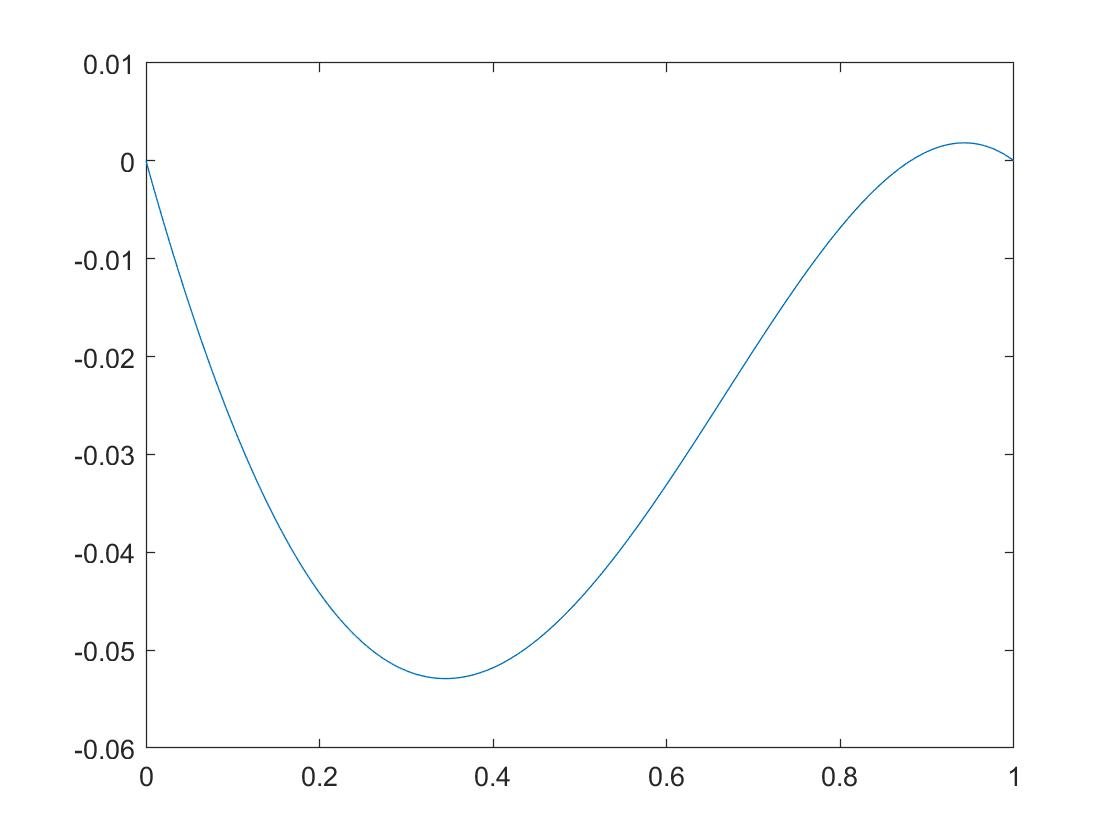
\includegraphics[height=0.4\textheight,width=0.8\linewidth]{2}
\caption{Result for test case 2.}
\end{figure}

Then, it's time to think about the convergence rate.
\begin{table}[H]
\centering
\begin{tabular}{|l|l|l|}
\hline
cycletimes & error & ratio\\\hline
1 & 0.609378&\\ \hline
2 & 0.176765& 3.4474\\ \hline
3 & 0.0372886& 4.74044\\ \hline
4 & 0.00701537& 5.31528\\ \hline
5 & 0.0012533& 5.59751\\ \hline
6 & 0.000218395& 5.7387\\ \hline
7 & 3.76241e-05& 5.80465\\ \hline
8 & 6.45586e-06& 5.82791\\ \hline
9 & 1.14953e-06& 5.61606\\ \hline
10 & 2.11361e-07& 5.43872\\ \hline
11 & 3.90696e-08& 5.40986\\ \hline
12 & 7.25591e-09& 5.38453\\ \hline
13 & 1.35293e-09& 5.36311\\ \hline
14 & 2.53106e-10& 5.34531\\ \hline
15 & 4.74813e-11& 5.33064\\ \hline
16 & 9.061e-12& 5.24018\\ \hline
17 & 1.72204e-12& 5.2618\\ \hline
18 & 3.59286e-13& 4.79294\\ \hline
19 & 3.01682e-13& 1.19094\\ \hline
20 & 2.66584e-13& 1.13166\\ \hline
21 & 2.69174e-13& 0.990378\\ \hline
22 & 3.22848e-13& 0.833748\\ \hline
23 & 3.60983e-13& 0.894359\\ \hline
24 & 3.84917e-13& 0.937819\\ \hline
25 & 2.87661e-13& 1.33809\\ \hline
26 & 2.69531e-13& 1.06726\\ \hline
27 & 2.35684e-13& 1.14362\\ \hline
28 & 2.35594e-13& 1.00038\\ \hline
29 & 3.60625e-13& 0.653294\\ \hline
30 & 2.66584e-13& 1.35276\\ \hline
31 & 3.12399e-13& 0.853345\\ \hline
32 & 3.58214e-13& 0.872102\\ \hline
\end{tabular}
\caption{Convergence rate for test case 2: n=128}
\end{table}
\begin{table}[H]
\centering
\begin{tabular}{|l|l|l|}
\hline
cycletimes & error & ratio\\\hline
1 & 0.658962&\\ \hline
2 & 0.236748& 2.78339\\ \hline
3 & 0.0568406& 4.16513\\ \hline
4 & 0.0116753& 4.86846\\ \hline
5 & 0.00222705& 5.24248\\ \hline
6 & 0.000408461& 5.4523\\ \hline
7 & 7.33232e-05& 5.5707\\ \hline
8 & 1.30133e-05& 5.63449\\ \hline
9 & 2.29746e-06& 5.66421\\ \hline
10 & 4.22718e-07& 5.43497\\ \hline
11 & 7.85543e-08& 5.38122\\ \hline
12 & 1.46312e-08& 5.36895\\ \hline
13 & 2.73216e-09& 5.35518\\ \hline
14 & 5.11537e-10& 5.34109\\ \hline
15 & 9.60167e-11& 5.32758\\ \hline
16 & 1.80657e-11& 5.31486\\ \hline
17 & 3.43035e-12& 5.26643\\ \hline
18 & 1.16632e-12& 2.94118\\ \hline
19 & 1.26641e-12& 0.920967\\ \hline
20 & 1.25203e-12& 1.01148\\ \hline
21 & 1.25856e-12& 0.994815\\ \hline
22 & 1.16747e-12& 1.07803\\ \hline
23 & 1.34057e-12& 0.870872\\ \hline
24 & 1.33158e-12& 1.00675\\ \hline
25 & 1.27655e-12& 1.04311\\ \hline
26 & 1.50574e-12& 0.847789\\ \hline
27 & 1.4859e-12& 1.01335\\ \hline
28 & 1.00953e-12& 1.47187\\ \hline
29 & 1.36253e-12& 0.740923\\ \hline
30 & 1.31517e-12& 1.03601\\ \hline
31 & 1.30838e-12& 1.00519\\ \hline
32 & 1.10001e-12& 1.18943\\ \hline
\end{tabular}
\caption{Convergence rate for test case 2:n=256}
\end{table}
\begin{table}[H]
\centering
\begin{tabular}{|l|l|l|}
\hline
cycletimes & error & ratio\\\hline
1 & 0.707978&\\ \hline
2 & 0.300924& 2.35268\\ \hline
3 & 0.0818& 3.67878\\ \hline
4 & 0.0183337& 4.46172\\ \hline
5 & 0.00373768& 4.9051\\ \hline
6 & 0.000722854& 5.17073\\ \hline
7 & 0.000135525& 5.33371\\ \hline
8 & 2.49428e-05& 5.43345\\ \hline
9 & 4.54123e-06& 5.49252\\ \hline
10 & 8.21984e-07& 5.52472\\ \hline
11 & 1.52312e-07& 5.39671\\ \hline
12 & 2.86672e-08& 5.31311\\ \hline
13 & 5.40008e-09& 5.30867\\ \hline
14 & 1.01854e-09& 5.30178\\ \hline
15 & 1.92398e-10& 5.29392\\ \hline
16 & 3.64145e-11& 5.28355\\ \hline
17 & 7.62115e-12& 4.77809\\ \hline
18 & 5.0182e-12& 1.5187\\ \hline
19 & 5.43848e-12& 0.92272\\ \hline
20 & 5.17313e-12& 1.05129\\ \hline
21 & 5.274e-12& 0.980875\\ \hline
22 & 4.90822e-12& 1.07452\\ \hline
23 & 5.32421e-12& 0.921868\\ \hline
24 & 5.04089e-12& 1.0562\\ \hline
25 & 5.99784e-12& 0.840451\\ \hline
26 & 5.19706e-12& 1.15408\\ \hline
27 & 5.01031e-12& 1.03727\\ \hline
28 & 5.52962e-12& 0.906086\\ \hline
29 & 6.1838e-12& 0.894211\\ \hline
30 & 5.51131e-12& 1.12202\\ \hline
31 & 4.76897e-12& 1.15566\\ \hline
32 & 5.47739e-12& 0.870664\\ \hline
\end{tabular}
\caption{Convergence rate for test case 3: n=512}
\end{table}
\begin{table}[H]
\centering
\begin{tabular}{|l|l|l|}
\hline
cycletimes & error & ratio\\\hline
1 & 0.771571&\\ \hline
2 & 0.364276& 2.11809\\ \hline
3 & 0.112375& 3.2416\\ \hline
4 & 0.027566& 4.07659\\ \hline
5 & 0.00601836& 4.58033\\ \hline
6 & 0.00122865& 4.89833\\ \hline
7 & 0.000240685& 5.10482\\ \hline
8 & 4.5928e-05& 5.24049\\ \hline
9 & 8.61798e-06& 5.32932\\ \hline
10 & 1.59999e-06& 5.38626\\ \hline
11 & 2.9515e-07& 5.42095\\ \hline
12 & 5.51994e-08& 5.34698\\ \hline
13 & 1.05192e-08& 5.24748\\ \hline
14 & 2.00364e-09& 5.25006\\ \hline
15 & 3.81569e-10& 5.25104\\ \hline
16 & 7.26316e-11& 5.25349\\ \hline
17 & 2.24543e-11& 3.23465\\ \hline
18 & 2.35891e-11& 0.951893\\ \hline
19 & 2.15705e-11& 1.09358\\ \hline
20 & 2.12576e-11& 1.01472\\ \hline
21 & 2.10873e-11& 1.00807\\ \hline
22 & 1.96407e-11& 1.07366\\ \hline
23 & 1.89702e-11& 1.03534\\ \hline
24 & 2.60157e-11& 0.729181\\ \hline
25 & 2.11269e-11& 1.2314\\ \hline
26 & 2.46901e-11& 0.855682\\ \hline
27 & 2.82618e-11& 0.873624\\ \hline
28 & 2.2346e-11& 1.26473\\ \hline
29 & 2.80491e-11& 0.796674\\ \hline
30 & 2.0995e-11& 1.33599\\ \hline
31 & 2.46901e-11& 0.850339\\ \hline
32 & 2.48985e-11& 0.991632\\ \hline
\end{tabular}
\caption{Convergence rate for test case 4: n=1024}
\end{table}

For homogenious problem, the performance of multigrid method is a little worse. I guess that it may be caused by the small disturb of boundary condition. But, it's still true that the convergence rate is nearly unrelated to the value of n. So the multigrid method is still work. 
\section{Statement}
In this answer file, I use full-weighting and linear operator to design the operator 
$I_{2h}^{h}$ and $I_{h}^{2h}$, and the initial guess is $\textbf{u}_{0}=\textbf{0}$
\end{document}